\subsection{Introduzione}
Questa sezione ha lo scopo di descrivere i vari casi d'uso\G{} che sono stati identificati dal gruppo \teamname{} come delle potenziali funzionalità dell'applicazione.

\subsection{Attori}
\begin{itemize}
    \item \textbf{Utente non registrato}: 
    è un utente che non ha ancora effettuato la registrazione presso l'applicativo.
    Non possiede credenziali per effettuare l'autenticazione presso la piattaforma e non ha accesso a nessuna funzionalità dell'applicazione;
    \item \textbf{Utente non autenticato}: 
    è un utente che ancora deve autenticarsi nell'applicazione. Può essere in possesso di credenziali di accesso oppure no;
    \item \textbf{Utente autenticato}:
    è un utente che ha effettuato l'autenticazione della piattaforma ed ha accesso alle funzionalità di essa.
\end{itemize}

\begin{figure}[!h]
    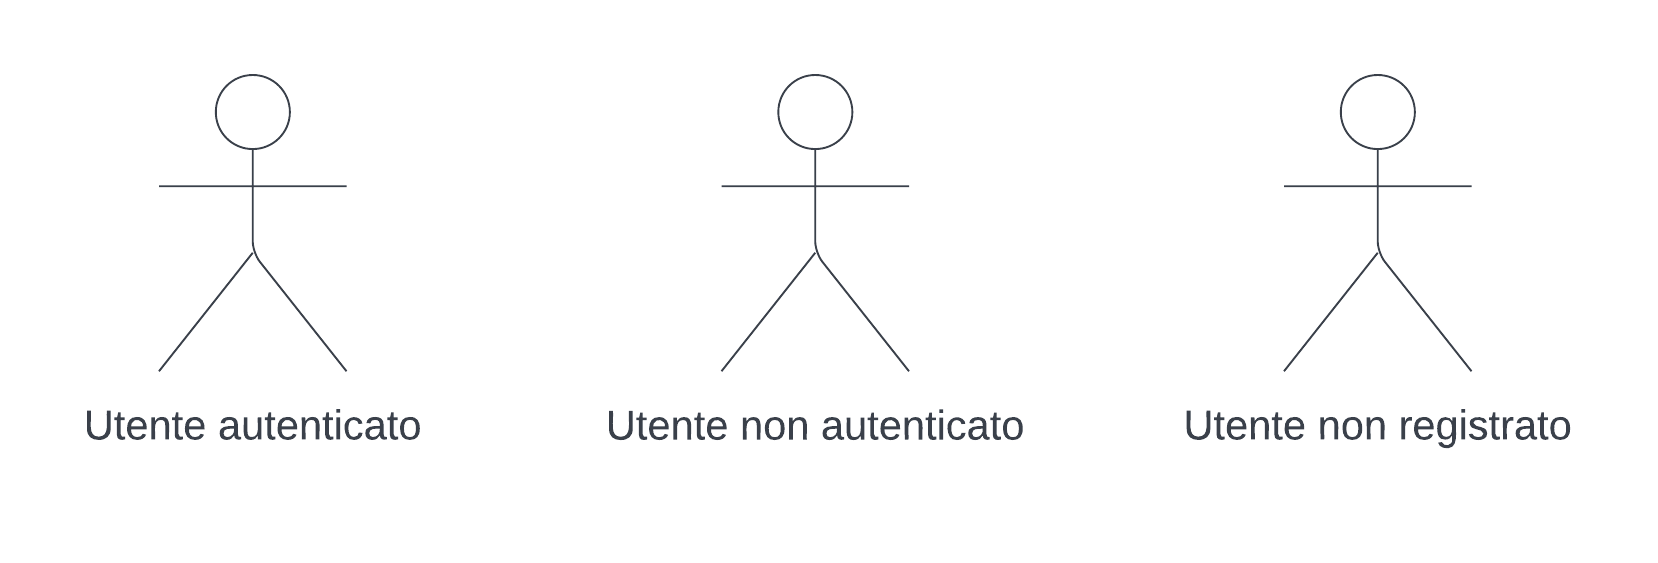
\includegraphics[width=10cm]{sezioni/Images/Actors.png}
    \centering
    \caption{Gerarchia attori}
\end{figure}
\newpage
    
\subsection{UC1 - Registrazione manuale}

\begin{figure}[!h]
    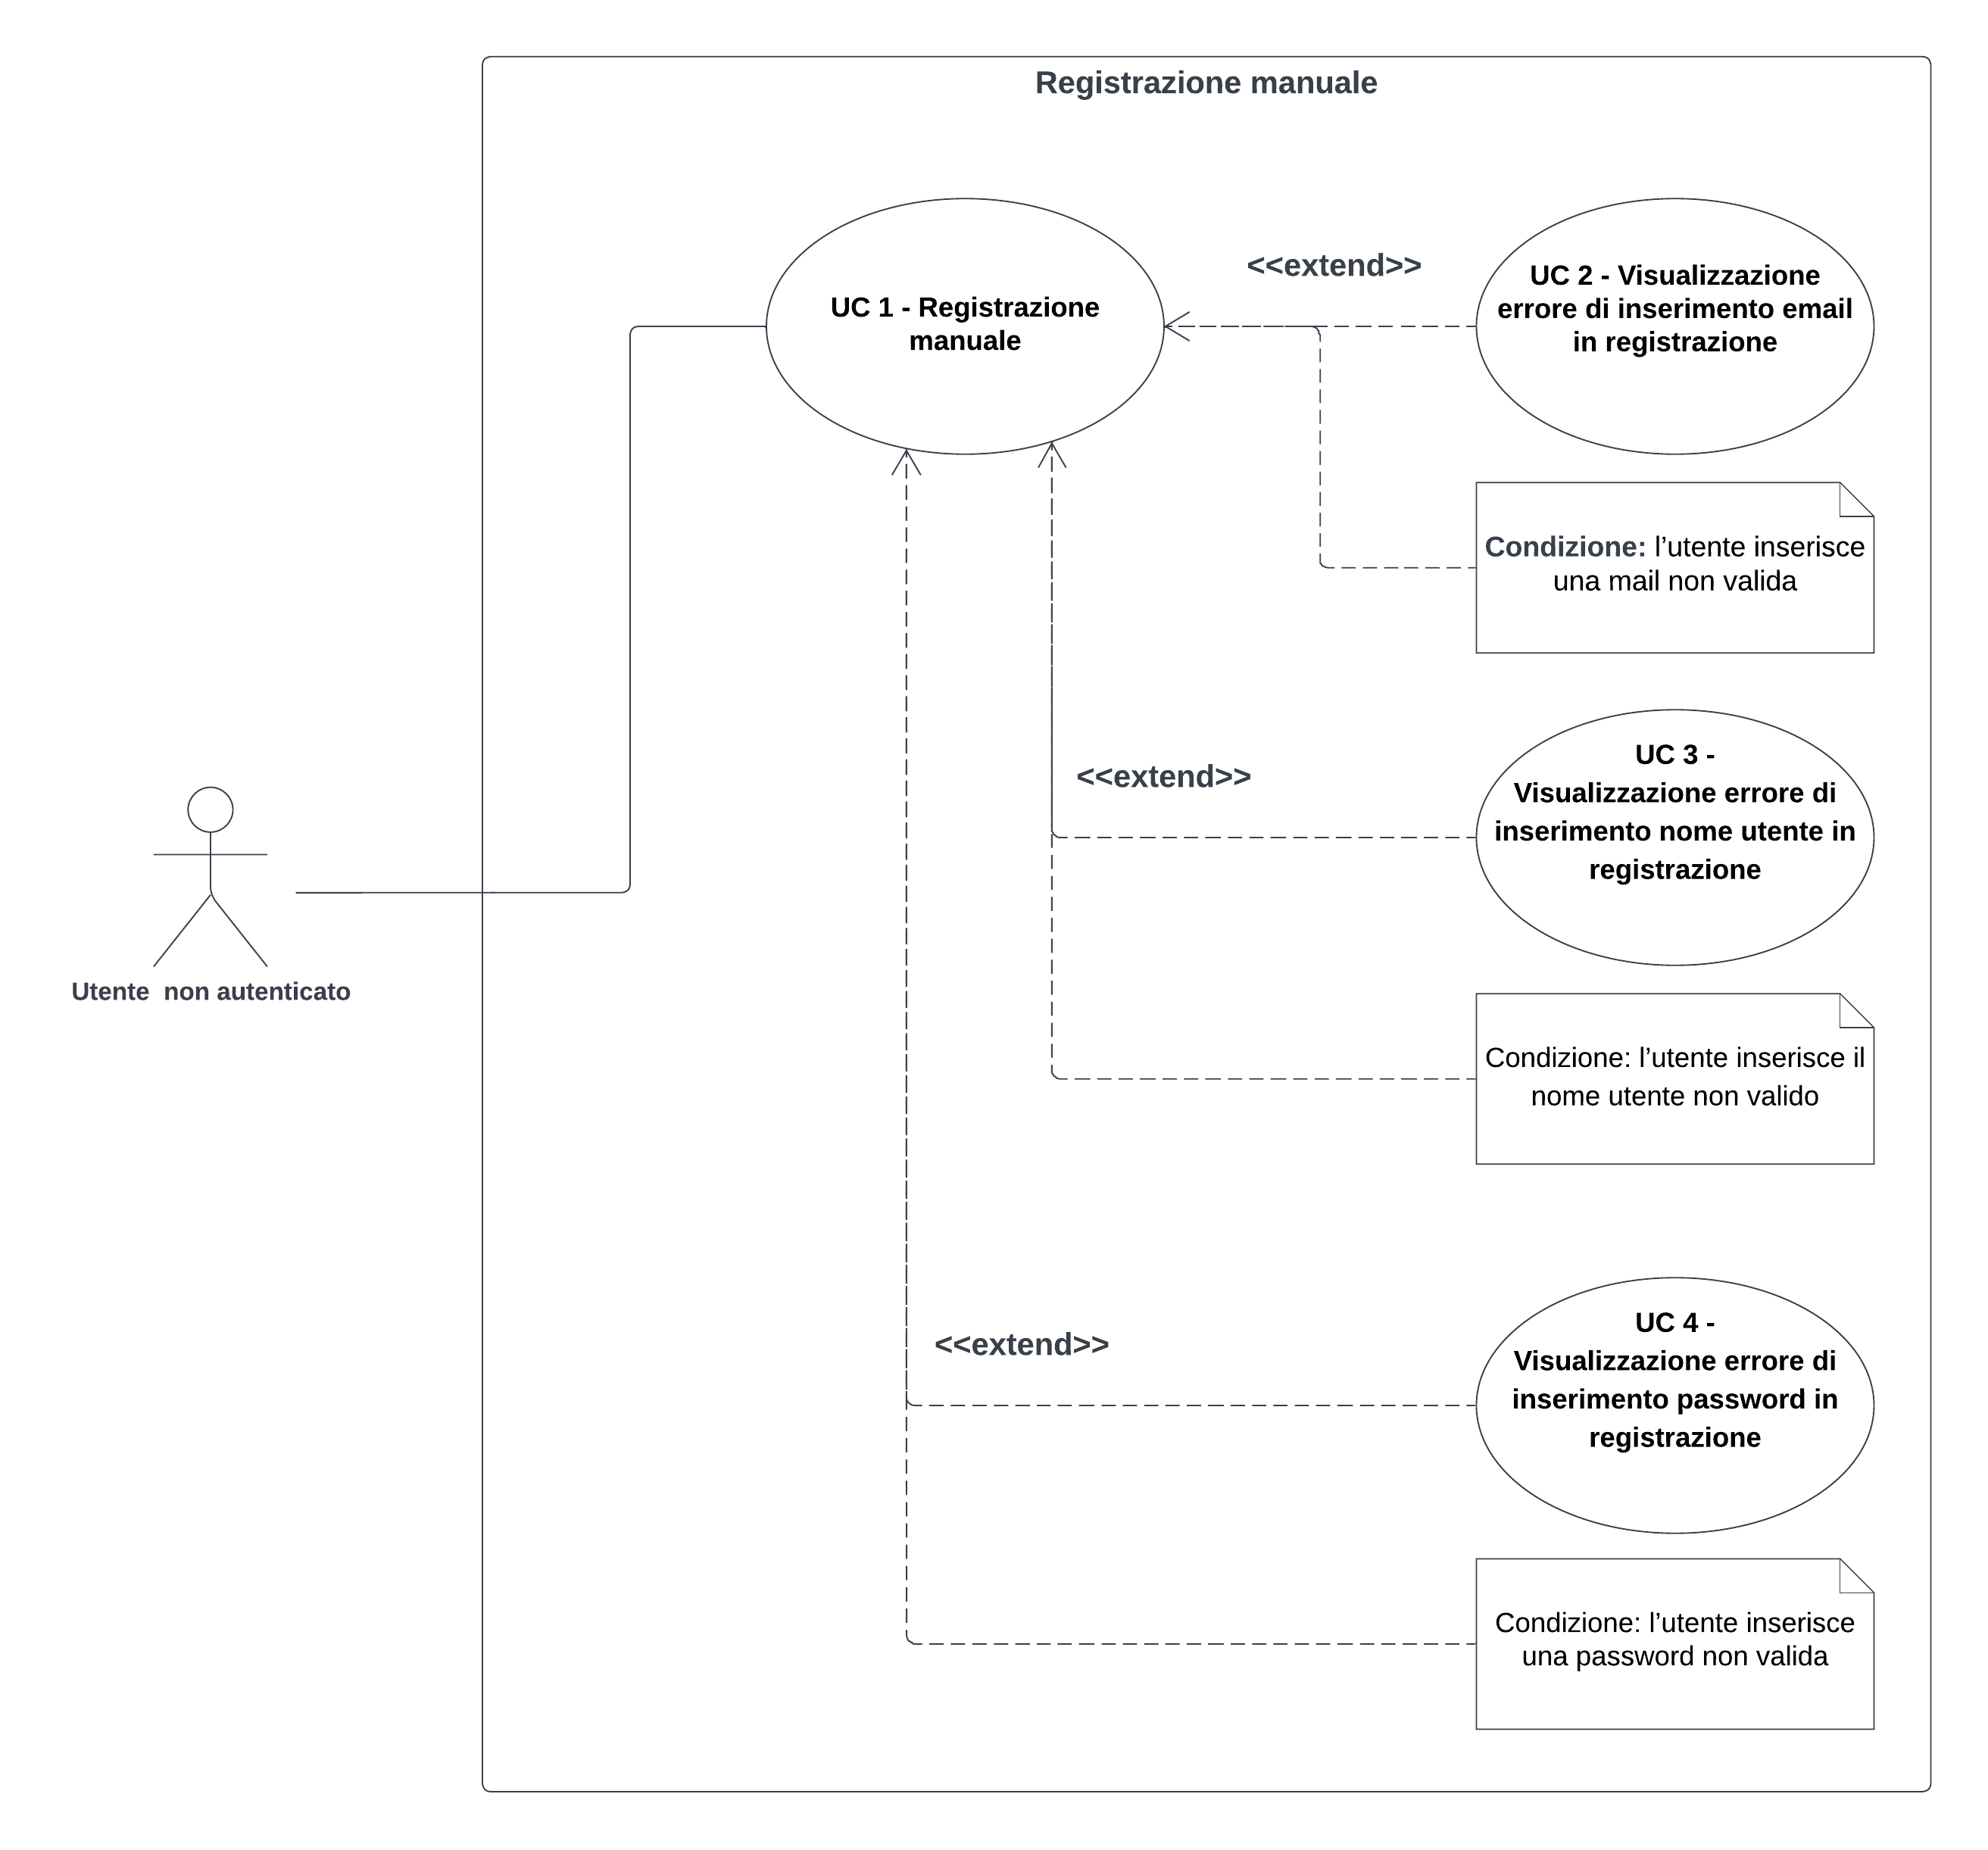
\includegraphics[width=15cm]{sezioni/Images/UC1.png}
    \centering
    \caption{UC1 - Registrazione manuale}
\end{figure}

\begin{itemize}
    \item \textbf{Attore}: utente non registrato.
    \item \textbf{Descrizione}: l'utente deve poter avere la possibilità di creare un account personale.
    \item \textbf{Scenario}:
    \begin{enumerate}
        \item l'utente si collega al sistema;
        \item l'utente clicca sul pulsante di registrazione;
        \item l'utente inserisce la propria email \textbf{(UC1.1)};
        \item l'utente inserisce il proprio nome utente \textbf{(UC1.2)};
        \item l'utente inserisce una password \textbf{(UC1.3)};
        \item l'utente conferma i dati inseriti per proseguire.
    \end{enumerate}
    \item \textbf{Estensioni}: 
        \begin{enumerate}
            \item l'utente inserisce una mail non valida  \textbf{(UC2)};
            \item l'utente inserisce il nome utente non valido \textbf{(UC3)};
            \item l'utente inserisce una password non valida \textbf{(UC4)}.
        \end{enumerate}

    \item \textbf{Precondizioni}: l'utente non è ancora registrato nel sistema.
    \item \textbf{Postcondizioni}: l'utente è registrato nel sistema.
\end{itemize}

\begin{figure}[!h]
    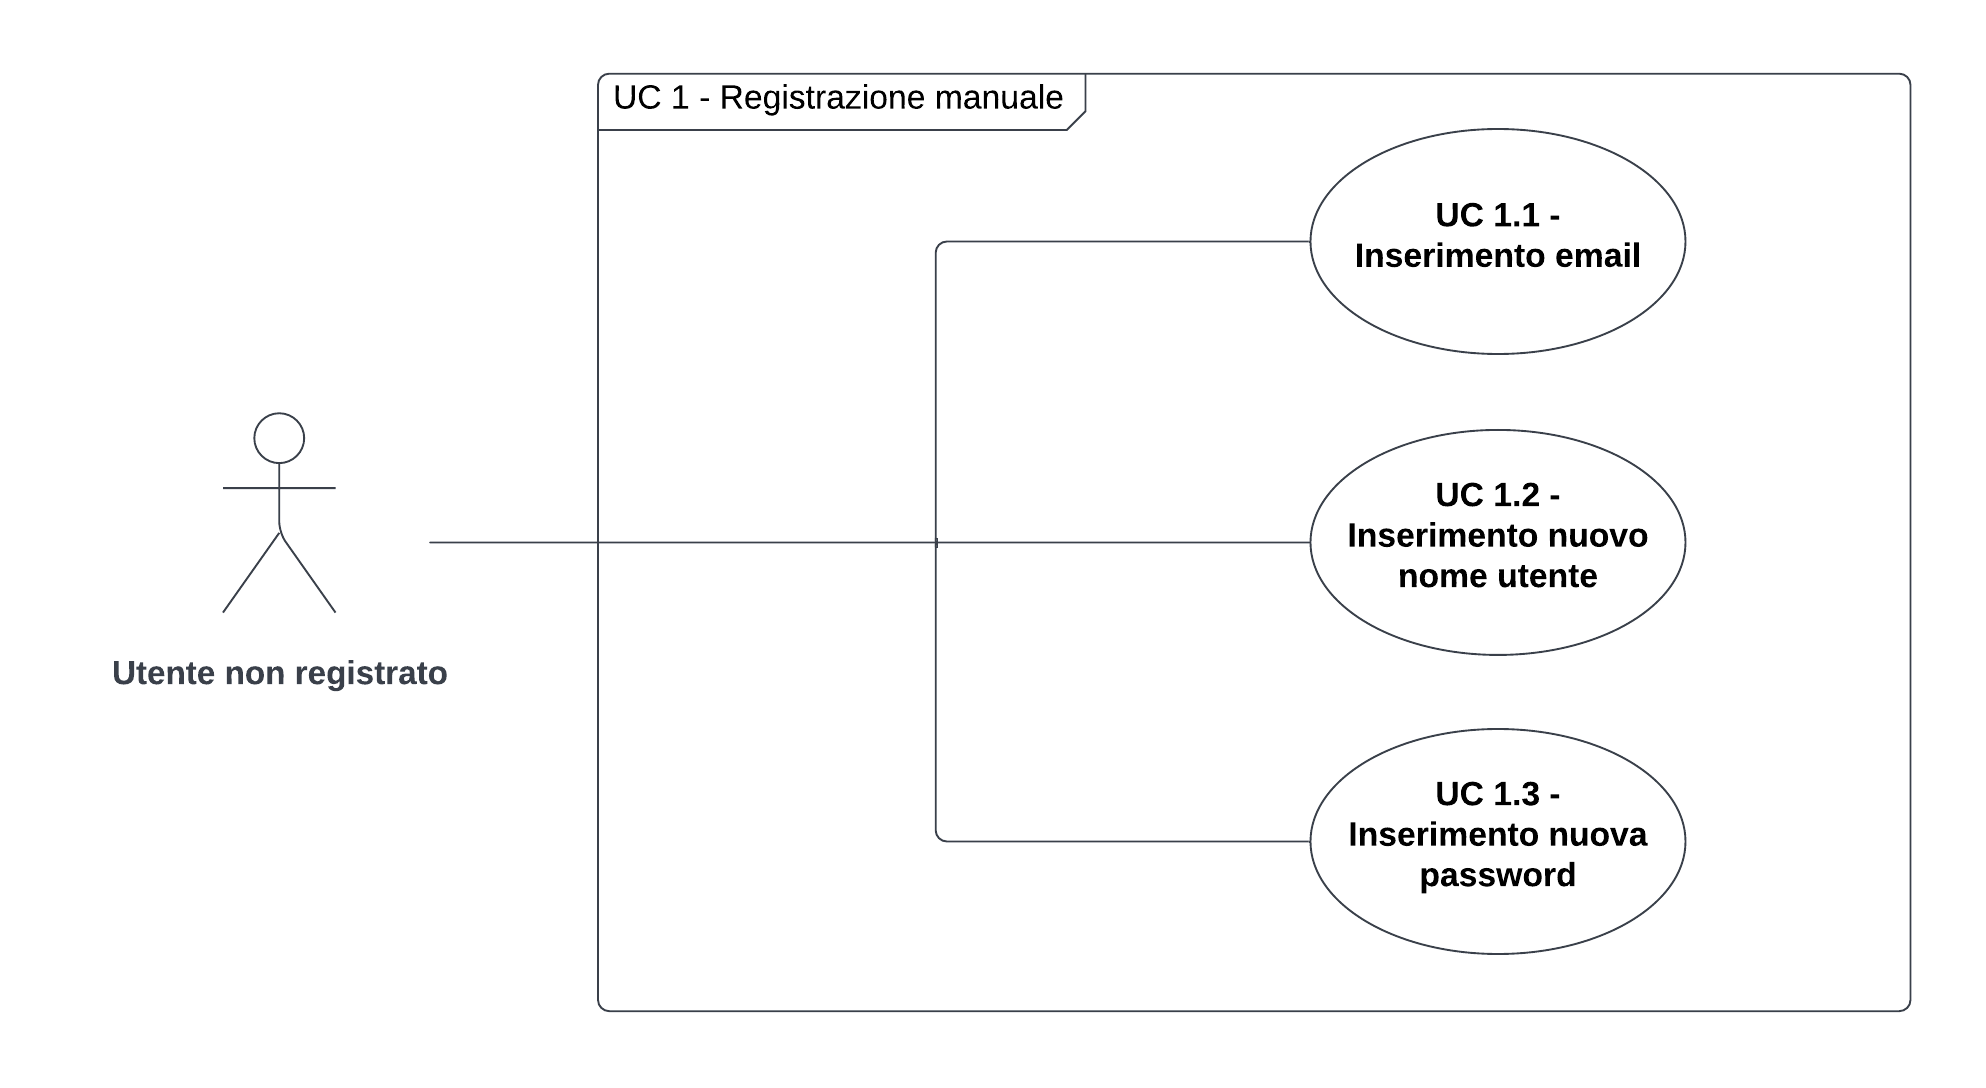
\includegraphics[width=15cm]{sezioni/Images/UC1_s.png}
    \centering
    \caption{Registrazione manuale}
\end{figure}

\subsubsection{UC1.1 - Inserimento email}
\begin{itemize}
    \item \textbf{Attore}: utente non registrato.
    \item \textbf{Descrizione}: l'utente deve avere la possibilità di inserire l'email.
    \item \textbf{Scenario}:
    \begin{enumerate}
        \item l'utente seleziona il campo relativo alla mail;
        \item l'utente inserisce la propria email.
    \end{enumerate}

    \item \textbf{Precondizioni}: l'utente effettua l'attività di registrazione.
    \item \textbf{Postcondizioni}: l'utente ha compilato il campo relativo alla mail.
\end{itemize}

\subsubsection{UC1.2 - Inserimento nuovo nome utente}
\begin{itemize}
    \item \textbf{Attore}: utente non registrato.
    \item \textbf{Descrizione}: l'utente deve avere la possibilità di creare un nuovo nome utente.
    \item \textbf{Scenario}:
    \begin{enumerate}
        \item l'utente seleziona il campo relativo il nuovo nome utente;
        \item l'utente crea il proprio nuovo nome utente.
    \end{enumerate}
    \item \textbf{Precondizioni}: l'utente effettua l'attività di registrazione.
    \item \textbf{Postcondizioni}: l'utente ha compilato il campo relativo il nuovo nome utente.
\end{itemize}

\subsubsection{UC1.3 - Inserimento nuova password}
\begin{itemize}
    \item \textbf{Attore}: utente non registrato.
    \item \textbf{Descrizione}: l'utente deve avere la possibilità di creare una nuova password.
    \item \textbf{Scenario}:
    \begin{enumerate}
        \item l'utente seleziona il campo relativo la nuova password;
        \item l'utente crea la nuova password.
    \end{enumerate}

    \item \textbf{Precondizioni}: l'utente effettua l'attività di registrazione.
    \item \textbf{Postcondizioni}: l'utente ha compilato il campo relativo la nuova password.
\end{itemize}

\subsection{UC2 - Visualizzazione errore di inserimento email in registrazione}
\begin{itemize}
    \item \textbf{Attore}: utente non registrato.
    \item \textbf{Descrizione}: l'utente deve essere notificato con un errore nel caso in cui le informazioni inserite nel campo email siano invalide.
    \item \textbf{Scenario}: l'utente visualizza un messaggio di errore.
    \item \textbf{Precondizioni}: l'utente inserisce una mail non valida nell'apposito input box.
    \item \textbf{Postcondizioni}: l'utente riceve il messaggio di errore.
\end{itemize}

\subsection{UC3 - Visualizzazione errore di inserimento nome utente in registrazione}
\begin{itemize}
    \item \textbf{Attore}: utente non registrato.
    \item \textbf{Descrizione}: l'utente deve essere notificato con un errore nel caso in cui venga inserito un nome utente non valido.
    \item \textbf{Scenario}: l'utente visualizza un messaggio di errore.
    \item \textbf{Precondizioni}: l'utente inserisce un nome utente non valido nell'apposito input box.
    \item \textbf{Postcondizioni}: l'utente riceve il messaggio di errore.
\end{itemize}

\subsection{UC4 - Visualizzazione errore di inserimento password in registrazione}
\begin{itemize}
    \item \textbf{Attore}: utente non registrato.
    \item \textbf{Descrizione}: l'utente deve essere notificato con un errore nel caso in cui inserisca una password non valida durante la fase di registrazione.
    \item \textbf{Scenario}: l'utente visualizza un messaggio di errore.
    \item \textbf{Precondizioni}: l'utente inserisce una password non valida nell'apposito input box.
    \item \textbf{Postcondizioni}: l'utente riceve il messaggio di errore.
\end{itemize}

\subsection{UC5 - Login}
\begin{figure}[!h]
    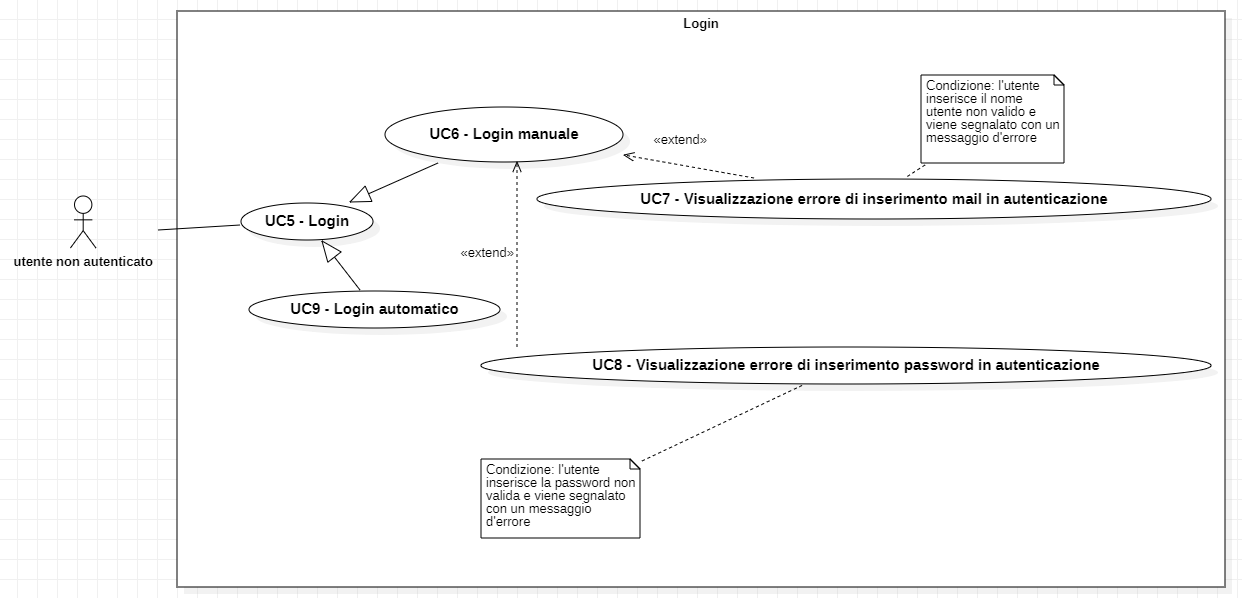
\includegraphics[width=15cm]{sezioni/Images/UC5-log.png}
    \centering
    \caption{UC5 - Login}
\end{figure}
\begin{itemize}
    \item \textbf{Attore}: l'utente non è autenticato.
    \item \textbf{Descrizione}: l'utente deve poter autenticarsi e accedere al proprio account.
    \item \textbf{Scenario}:
    \begin{enumerate}
        \item l'utente si collega al sistema;
        \item l'utente clicca sul pulsante di login;
        \item l'utente si collega manualmente \textbf{(UC6)} oppure automaticamente \textbf{(UC9)}.
    \end{enumerate}
    \item \textbf{Precondizioni}: l'utente non è ancora autenticato al sistema.
    \item \textbf{Postcondizioni}: l'utente si è autenticato al sistema.
\end{itemize}

\subsection{UC6 - Login manuale}

\begin{itemize}
    \item \textbf{Attore}: l'utente non è autenticato.
    \item \textbf{Descrizione}: l'utente accedendo con l'account personale, deve poter autenticarsi.
    \item \textbf{Scenario}:
    \begin{enumerate}
        \item l'utente si collega al sistema;
        \item l'utente clicca sul pulsante di login;
        \item l'utente inserisce il proprio nome utente \textbf{(UC6.1)};
        \item l'utente inserisce la propria password \textbf{(UC6.2)};
        \item l'utente decide se memorizzare la sessione \textbf{(UC6.3 )};
        \item l'utente clicca il pulsante di conferma per proseguire.
    \end{enumerate}
    \item \textbf{Estensioni}:
        \begin{enumerate}
            \item l'utente inserisce il nome utente non valido e viene segnalato con un messaggio d'errore \textbf{(UC 7)};
            \item l'utente inserisce la password non valida e viene segnalato con un messaggio d'errore \textbf{(UC 8)};
        \end{enumerate}

    \item \textbf{Precondizioni}: l'utente non è ancora autenticato.
    \item \textbf{Postcondizioni}: l'utente si è autenticato al sistema.
\end{itemize}

\begin{figure}[!h]
    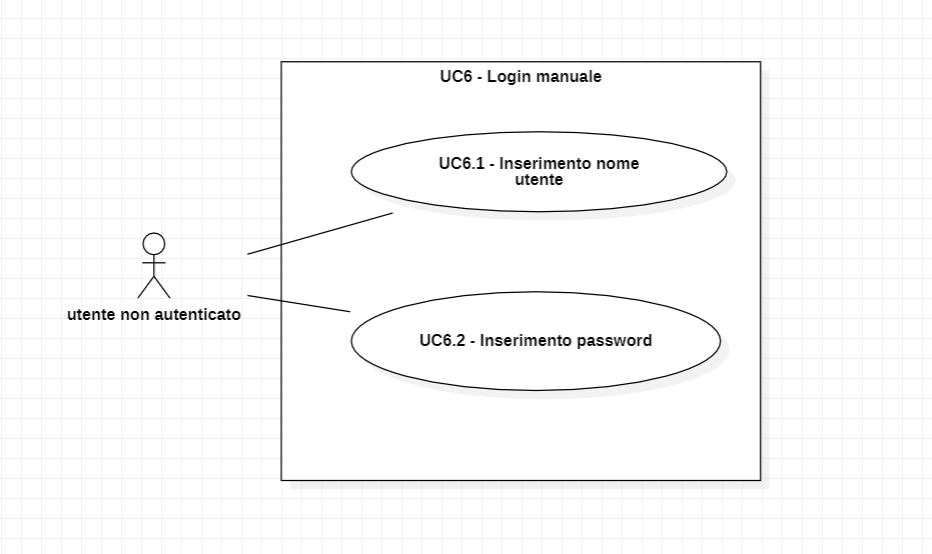
\includegraphics[width=10cm]{sezioni/Images/UC6-Manuale.png}
    \centering
    \caption{UC6 - Login manuale}
\end{figure}

\subsubsection{UC6.1 - Inserimento nome utente}
\begin{itemize}
    \item \textbf{Attore}: utente non autenticato.
    \item \textbf{Descrizione}: l'utente deve poter inserire il nome utente per autenticarsi.
    \item \textbf{Scenario}:
    \begin{enumerate}
        \item l'utente seleziona il campo relativo al nome utente;
        \item l'utente inserisce il nome utente.
    \end{enumerate}
    \item \textbf{Precondizioni}: l'utente effettua l'attività di autenticazione.
    \item \textbf{Postcondizioni}: l'utente ha compilato il campo relativo il nome utente.
\end{itemize}

\subsubsection{UC6.2 - Inserimento password}
\begin{itemize}
    \item \textbf{Attore}: utente non autenticato.
    \item \textbf{Descrizione}: l'utente deve poter inserire la password per autenticarsi.
    \item \textbf{Scenario}:
    \begin{enumerate}
        \item l'utente seleziona il campo relativo alla password;
        \item l'utente inserisce la password.
    \end{enumerate}

    \item \textbf{Precondizioni}: l'utente effettua l'attività di autenticazione.
    \item \textbf{Postcondizioni}: l'utente ha compilato il campo relativo il nome utente.
\end{itemize}

\subsubsection{UC6.3 Memorizzazione sessione}
\begin{itemize}
    \item \textbf{Attore}: utente non autenticato.
    \item \textbf{Descrizione}: l'utente deve poter memorizzare la sessione.
    \item \textbf{Scenario}: l'utente spunta la casella per mantenere memorizzata la sessione.
    \item \textbf{Precondizioni}: l'utente effettua l'attività di autenticazione.
    \item \textbf{Postcondizioni}: l'utente ha chiesto che la sessione venga memorizzata.
\end{itemize}

\subsection{UC7 - Visualizzazione errore di inserimento mail in autenticazione}
\begin{itemize}
    \item \textbf{Attore}: utente non autenticato.
    \item \textbf{Descrizione}: l'utente deve essere notificato con un errore nel caso in cui l'email inserita sia invalida durante la fase di autenticazione.
    \item \textbf{Scenario}: l'utente visualizza un messaggio di errore. 
    \item \textbf{Precondizioni}: l'utente effettua l'attività di autenticazione ed inserisce l'email non valida.
    \item \textbf{Postcondizioni}: l'utente riceve il messaggio di errore.
\end{itemize}

\subsection{UC8 - Visualizzazione errore di inserimento password in autenticazione} 
\begin{itemize}
    \item \textbf{Attore}: utente non autenticato.
    \item \textbf{Descrizione}: l'utente deve essere notificato con un errore nel caso in cui la password inserita sia invalida durante la fase di autenticazione.
    \item \textbf{Scenario}: l'utente visualizza un messaggio di errore. 
    \item \textbf{Precondizioni}: l'utente effettua l'attività di autenticazione ed inserisce la password non valida.
    \item \textbf{Postcondizioni}: l'utente riceve il messaggio di errore.
\end{itemize}

\subsection{UC9 - Login automatico}
\begin{itemize}
    \item \textbf{Attore}: utente non autenticato.
    \item \textbf{Descrizione}: l'utente accedendo con l'account personale, deve poter autenticarsi automaticamente se la sessione rimane memorizzata.
    \item \textbf{Scenario}:
    \begin{enumerate}
        \item l'utente si collega al sistema;
        \item l'utente viene automaticamente autenticato.
    \end{enumerate}

    \item \textbf{Precondizioni}: l'utente ha una sessione attiva memorizzata.
    \item \textbf{Postcondizioni}: l'utente si è autenticato al sistema.
\end{itemize}

\subsection{UC10 - Logout}
\begin{itemize}
    \item \textbf{Attore}: l'utente è autenticato.
    \item \textbf{Descrizione}: l'utente deve poter uscire dalla sessione.
    \item \textbf{Scenario}:
    \begin{enumerate}
        \item l'utente è collegato al sistema;
        \item l'utente clicca il pulsante di logout.
    \end{enumerate}

    \item \textbf{Precondizioni}: l'utente è autenticato.
    \item \textbf{Postcondizioni}: l'utente non è più autenticato al sistema.
\end{itemize}

\subsection{UC11 - Modifica password}

\begin{figure}[H]
    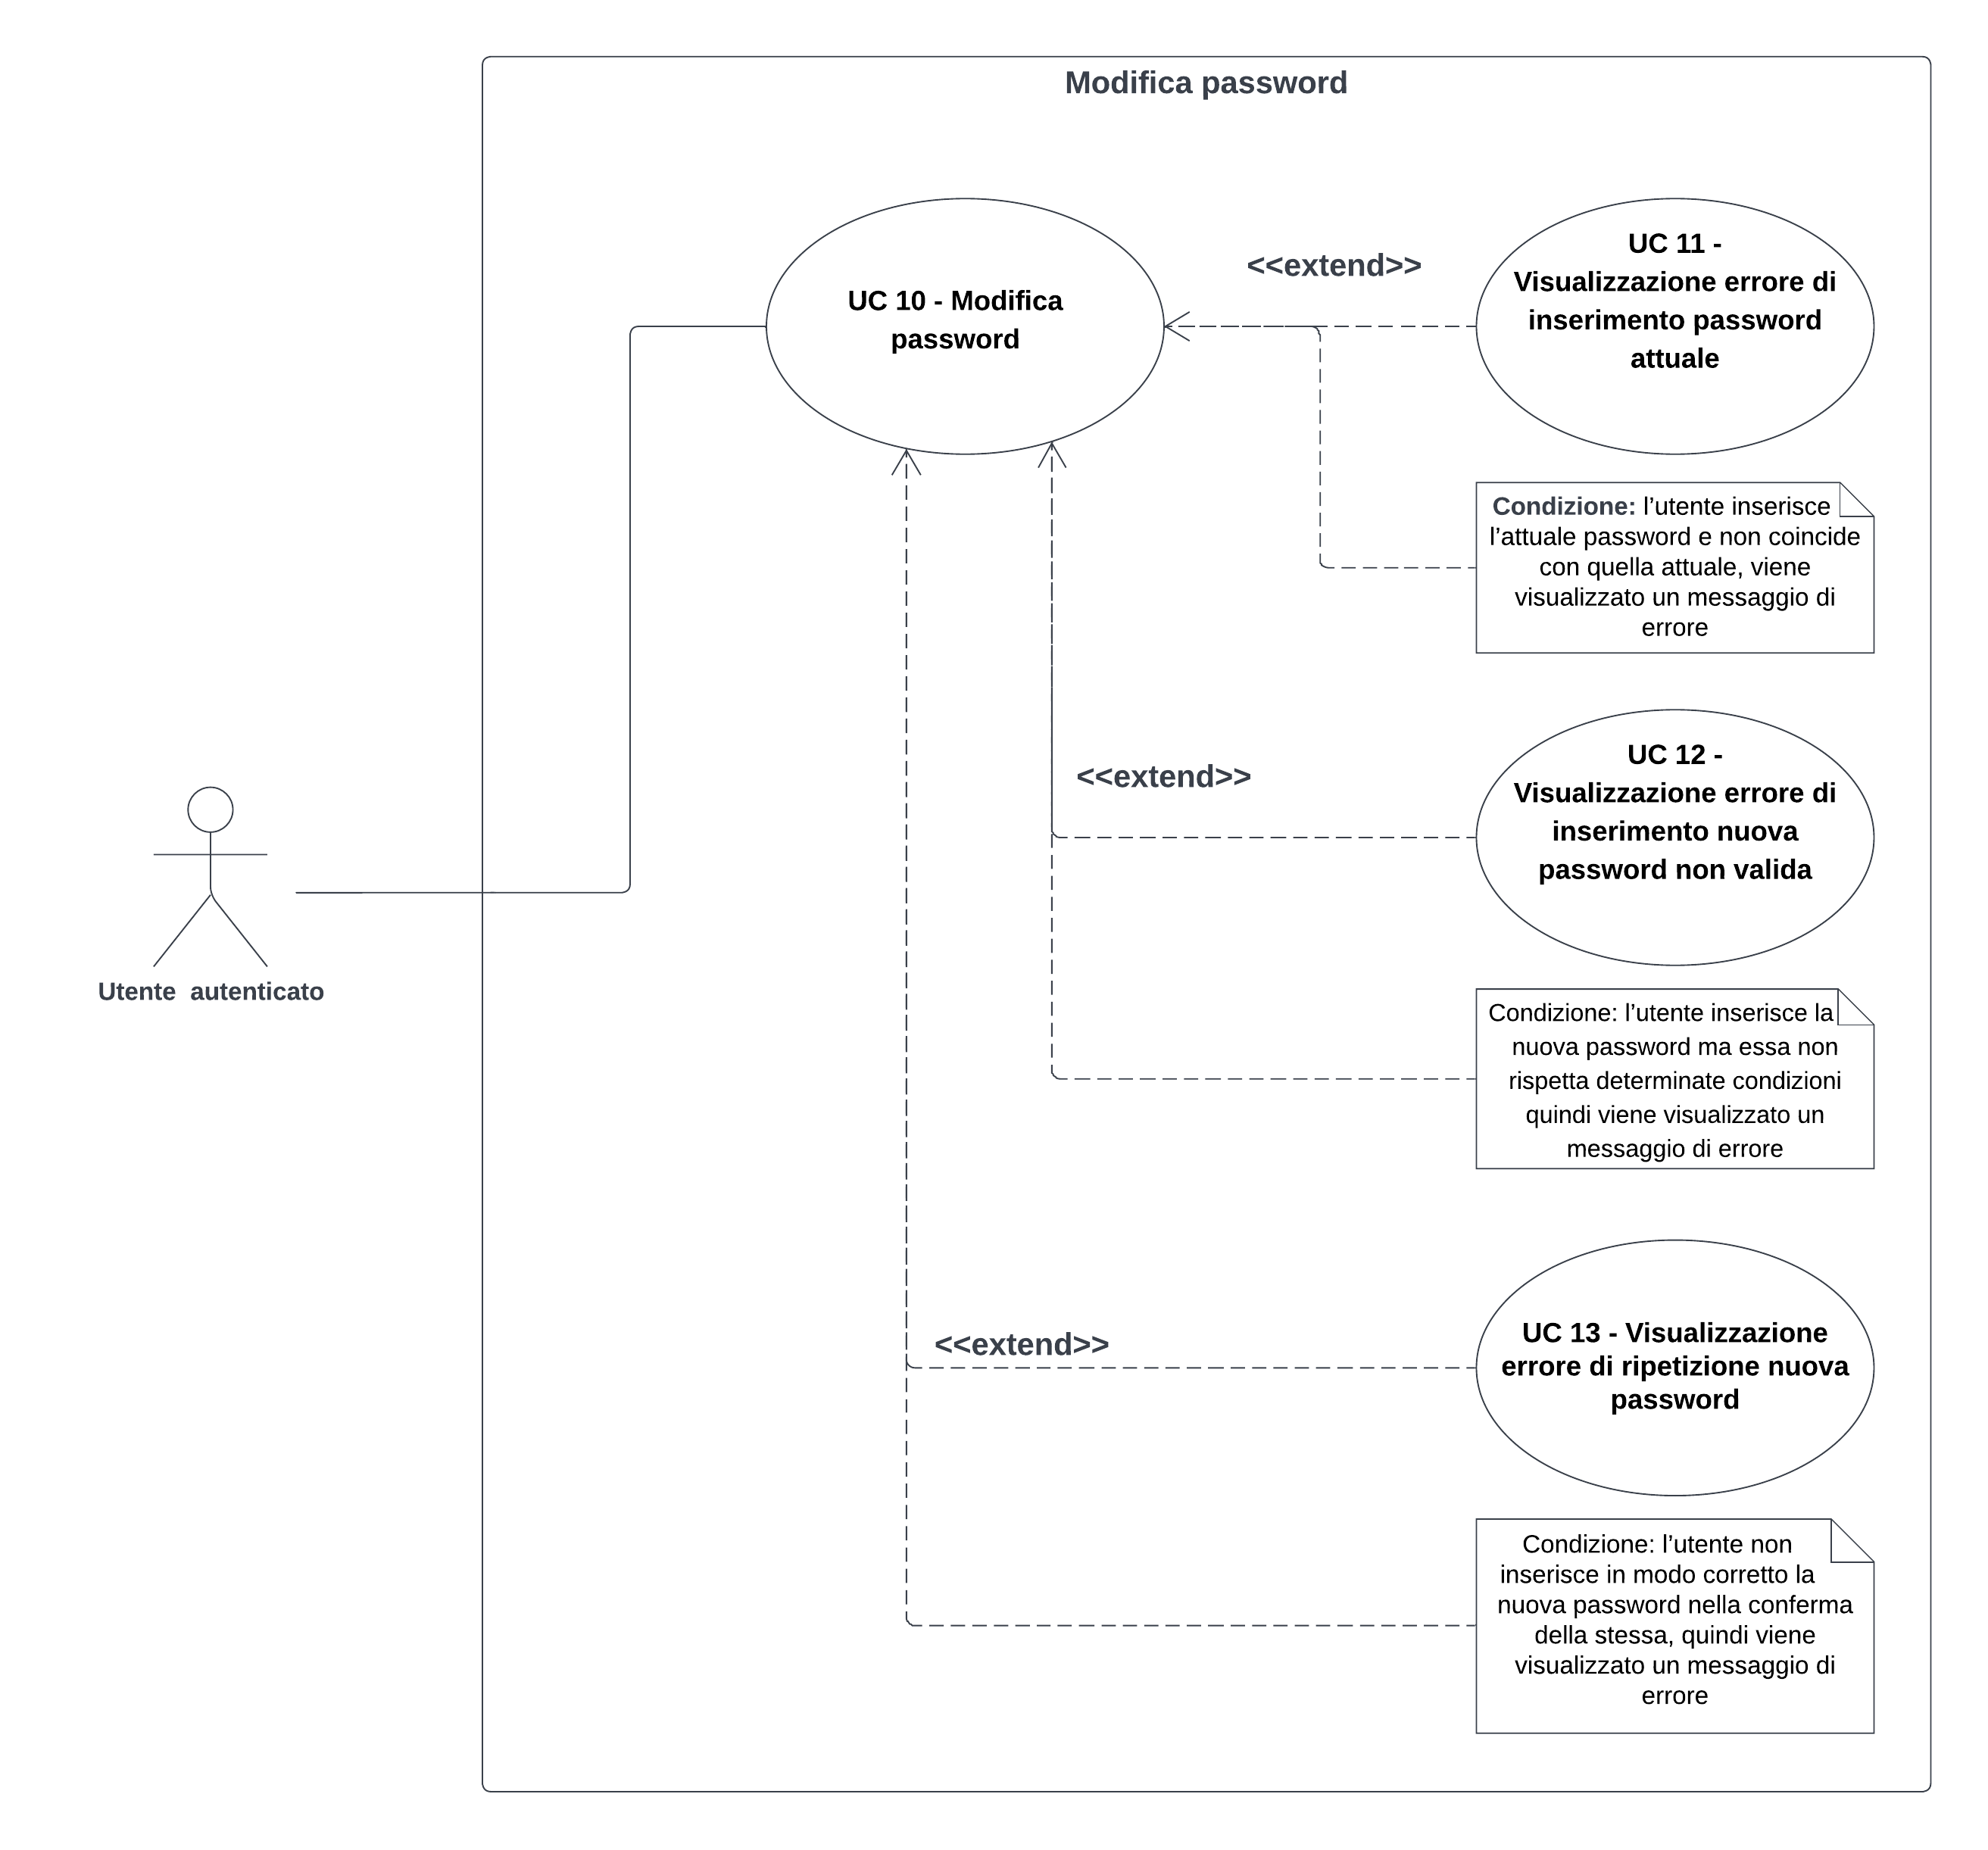
\includegraphics[width=15cm]{sezioni/Images/UC10.png}
    \centering
    \caption{Modifica password}
\end{figure}

\begin{itemize}
    \item \textbf{Attore}: l'utente è autenticato.
    \item \textbf{Descrizione}: l'utente deve poter modificare l'attuale password, con la quale effettua il login.
    \item \textbf{Scenario}:
    \begin{enumerate}
        \item inserimento password attuale;
        \item inserimento nuova password;
        \item conferma nuova password;
        \item conferma modifica password.
    \end{enumerate}
    \textbf{Estensioni}:
    \begin{enumerate}
        \item l'utente inserisce l'attuale password e non coincide con quella attuale, viene visualizzato un messaggio di errore \textbf{(UC12)};
        \item l'utente inserisce la nuova password ma essa non rispetta determinate condizioni quindi viene visualizzato un messaggio di errore \textbf{(UC13)};
        \item l'utente non inserisce in modo corretto la nuova password nella conferma della stessa, quindi viene visualizzato un messaggio di errore \textbf{(UC14)};
    \end{enumerate}

    \item \textbf{Precondizioni}: l'utente è autenticato con una determinata password.
    \item \textbf{Postcondizioni}: l'utente è autenticato con una nuova password.
\end{itemize}

\begin{figure}[!h]
    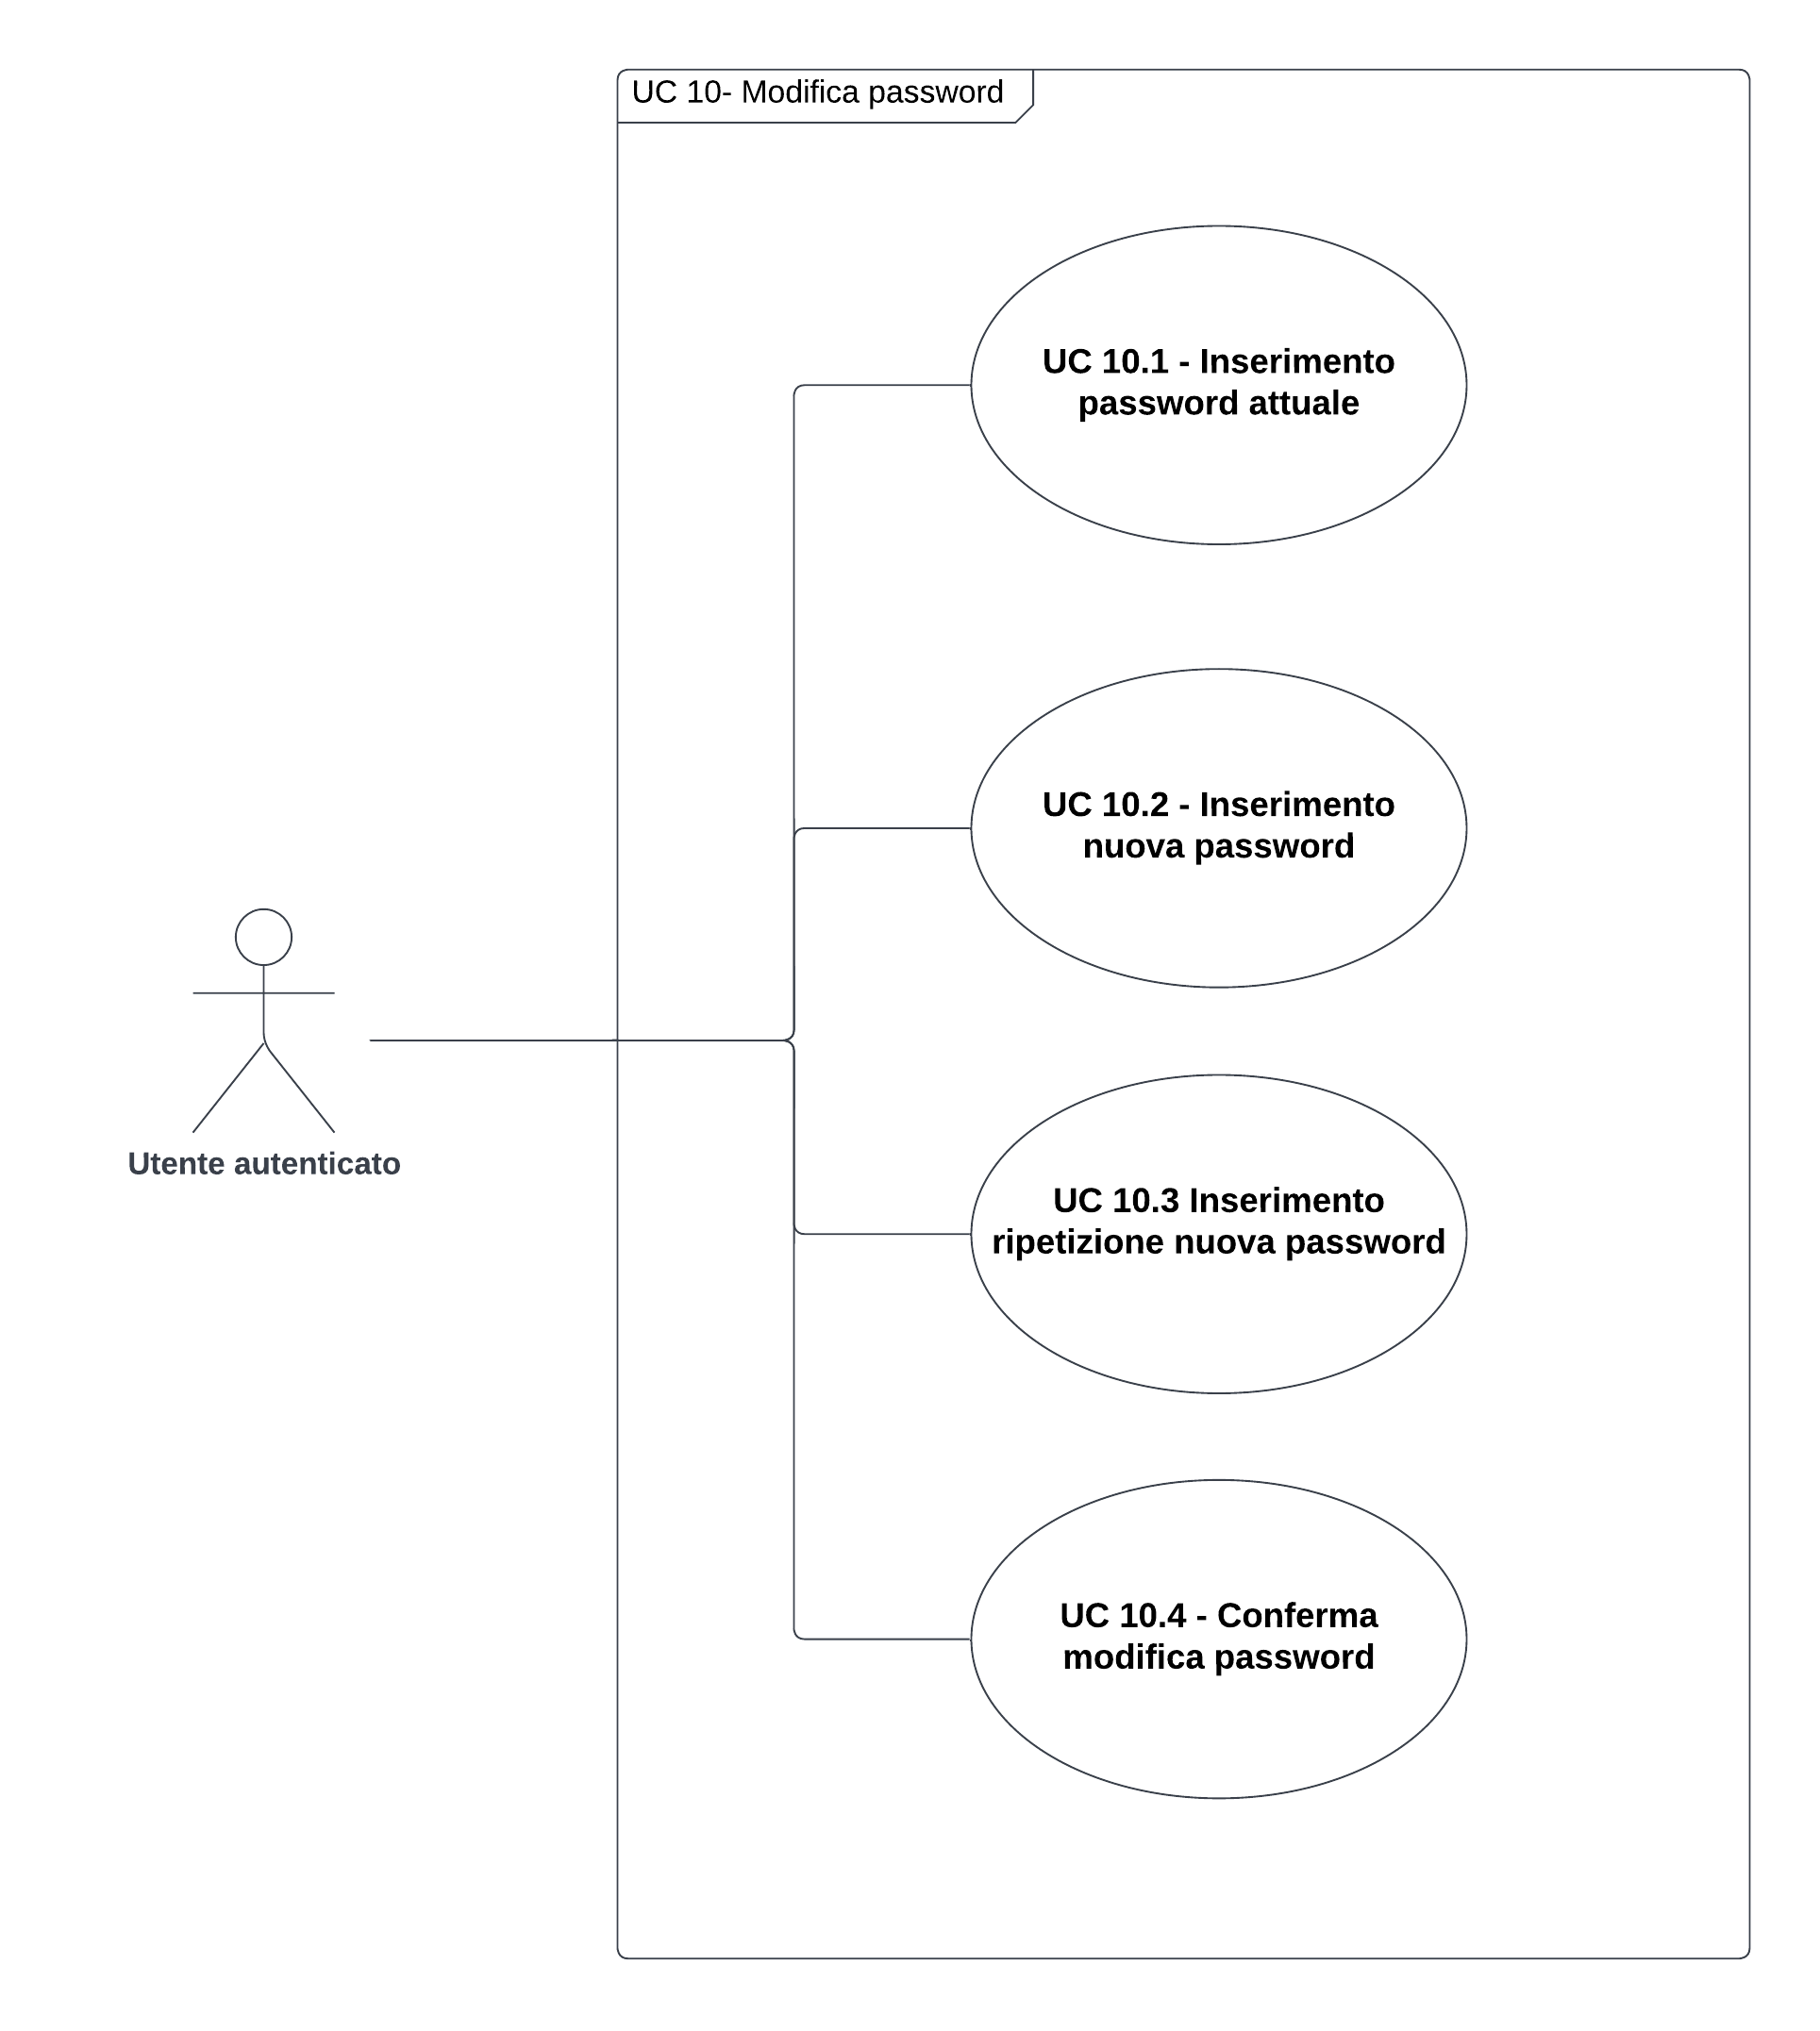
\includegraphics[width=15cm]{sezioni/Images/UC10_s.png}
    \centering
    \caption{Modifica password}
\end{figure}

\subsubsection{UC11.1 - Inserimento password attuale} 
\begin{itemize}
    \item \textbf{Attore}: l'utente è autenticato.
    \item \textbf{Descrizione}: l'utente deve inserire la password attuale durante la sessione di “modifica password”.
    \item \textbf{Scenario}:
    \begin{enumerate}
        \item l'utente seleziona il campo riferito alla password attuale;
        \item l'utente inserisce la password attuale.
    \end{enumerate}

    \item \textbf{Precondizioni}: l'utente svolge la sessione di modifica password.
    \item \textbf{Postcondizioni}: l'utente ha inserito la propria password attuale.

\end{itemize}

\subsubsection{UC11.2 - Inserimento nuova password}
\begin{itemize}
    \item \textbf{Attore}: l'utente è autenticato.
    \item \textbf{Descrizione}: durante l'attività di modifica della password l'utente deve poter inserire la nuova password.
    \item \textbf{Scenario}:
    \begin{enumerate}
        \item l'utente seleziona il campo riferito alla nuova password;
        \item l'utente inserisce la nuova password.
    \end{enumerate}

    \item \textbf{Precondizioni}: l'utente svolge la sessione di modifica password.
    \item \textbf{Postcondizioni}: l'utente ha inserito la nuova password.
\end{itemize}

\subsubsection{UC11.3 - Inserimento ripetizione nuova password}
\begin{itemize}
    \item \textbf{Attore}: l'utente è autenticato.
    \item \textbf{Descrizione}: durante l'attività di modifica password l'utente deve poter inserire la ripetizione della nuova password.
    \item \textbf{Scenario}:
    \begin{enumerate}
        \item l'utente seleziona il campo riferito alla ripetizione della nuova password;
        \item l'utente inserisce la ripetizione della nuova password.
    \end{enumerate}

    \item \textbf{Precondizioni}: l'utente svolge la sessione di modifica password.
    \item \textbf{Postcondizioni}: l'utente ha inserito la ripetizione della nuova password.
\end{itemize}

\subsubsection{UC11.4 - Conferma modifica password}
\begin{itemize}
    \item \textbf{Attore}: l'utente è autenticato.
    \item \textbf{Descrizione}: durante l'attività di modifica password l'utente deve poter confermare la nuova password.
    \item \textbf{Scenario}: l'utente conferma la nuova password inserita. 
    \item \textbf{Precondizioni}: l'utente svolge la sessione di modifica password.
    \item \textbf{Postcondizioni}: l'utente ha provato a modificare la propria password.
\end{itemize}

\subsection{UC12 - Visualizzazione errore di inserimento password attuale}
\begin{itemize}
    \item \textbf{Attore}: l'utente è autenticato.
    \item \textbf{Descrizione}: durante l'attività di modifica password l'utente deve ricevere un messaggio d'errore se l'inserimento della password attuale non è andato a buon fine.
    \item \textbf{Scenario}: l'utente legge un messaggio d'errore. 
    \item \textbf{Precondizioni}: l'utente svolge la sessione di modifica password e la password attuale inserita non è corretta.
    \item \textbf{Postcondizioni}: l'utente ha ricevuto un messaggio d'errore.
\end{itemize}

\subsection{UC13 - Visualizzazione errore di inserimento nuova password non valida}
\begin{itemize}
    \item \textbf{Attore}: l'utente è autenticato.
    \item \textbf{Descrizione}: durante l'attività di modifica password l'utente deve ricevere un messaggio d'errore se l'inserimento di una nuova password non è valida.
    \item \textbf{Scenario}: l'utente legge un messaggio d'errore. 
    \item \textbf{Precondizioni}: l'utente svolge la sessione di modifica password e la nuova password inserita non è valida.
    \item \textbf{Postcondizioni}: l'utente ha ricevuto un messaggio d'errore.

\end{itemize}

\subsection{UC14 - Visualizzazione errore di ripetizione nuova password}
\begin{itemize}
    \item \textbf{Attore}: l'utente è autenticato.
    \item \textbf{Descrizione}: durante l'attività di modifica password l'utente deve ricevere un messaggio d'errore se l'inserimento della ripetizione della nuova password non è uguale alla nuova password.
    \item \textbf{Scenario}: l'utente legge un messaggio d'errore. 
    \item \textbf{Precondizioni}: l'utente svolge la sessione di modifica password e la ripetizione della nuova password inserita non è corretta.
    \item \textbf{Postcondizioni}: l'utente ha ricevuto un messaggio d'errore.
\end{itemize}

\subsection{UC15 - Visualizzazione guida}

\begin{figure}[H]
    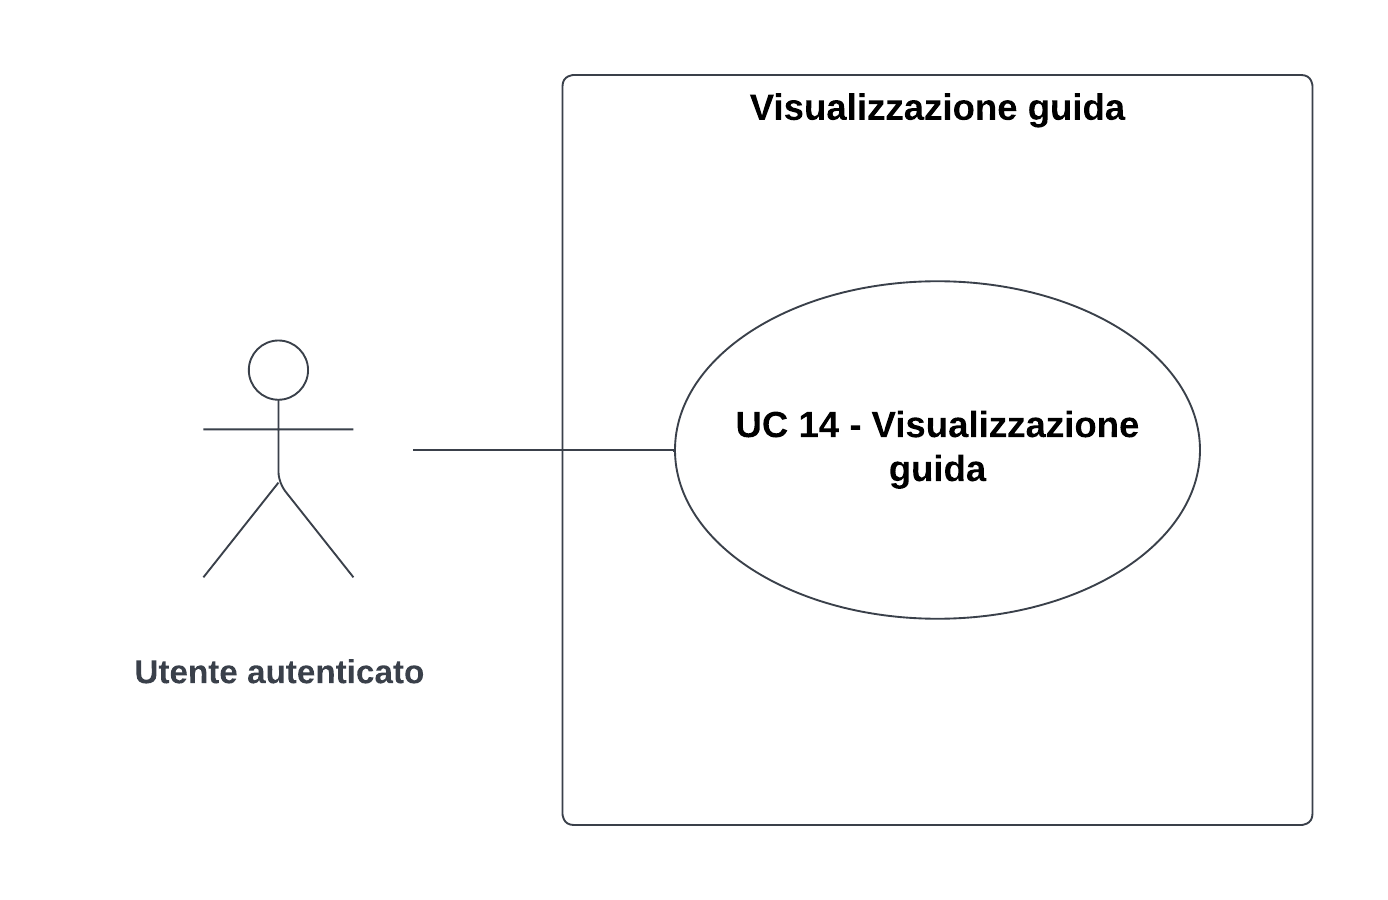
\includegraphics[width=10cm]{sezioni/Images/UC14.png}
    \centering
    \caption{Visualizzazione guida}
\end{figure}

\begin{itemize}
    \item \textbf{Attore}: l'utente è autenticato.
    \item \textbf{Descrizione}: l'utente deve poter visualizzare la guida in formato mappa o formato lista.
    \item \textbf{Scenario}: l'utente si trova nella home.
    \item \textbf{Precondizioni}: l'utente vuole visualizzare la guida.
    \item \textbf{Postcondizioni}: l'utente visualizza la guida.
\end{itemize}

\begin{figure}[H]
    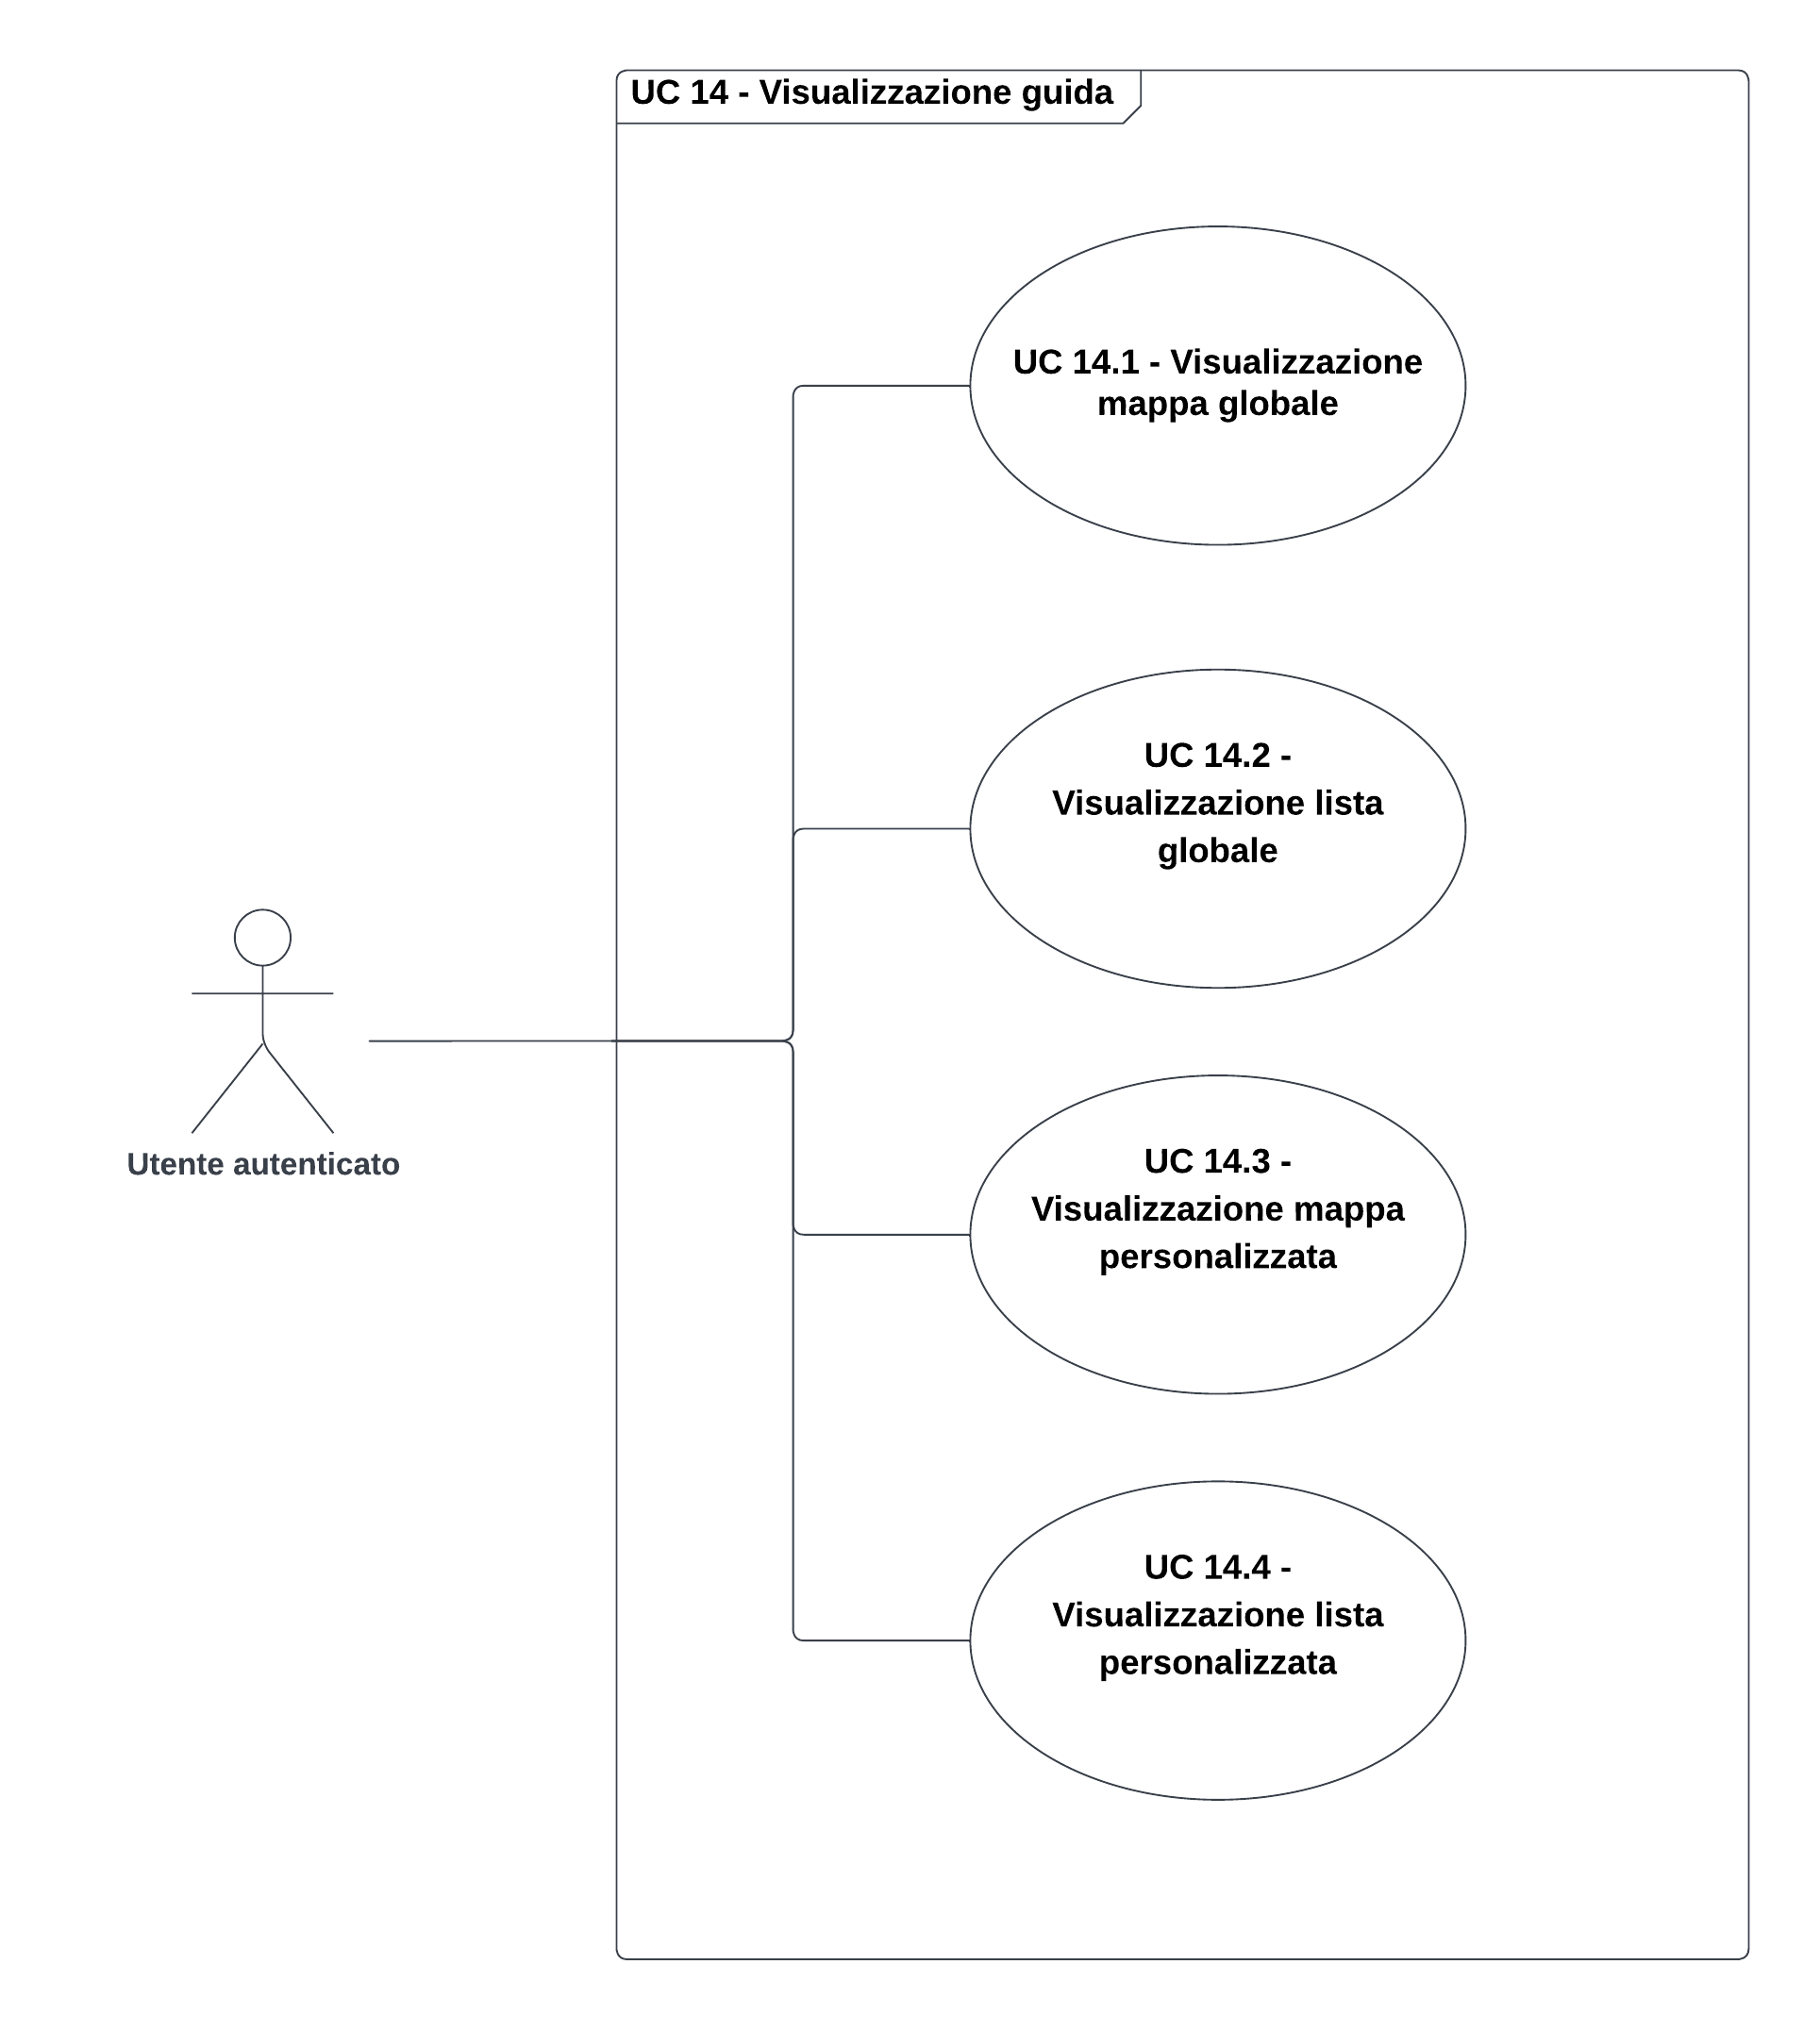
\includegraphics[width=13cm]{sezioni/Images/UC14_s.png}
    \centering
    \caption{Visualizzazione guida}
\end{figure}

\subsubsection{UC15.1 - Visualizzazione mappa globale}
\begin{itemize}
    \item \textbf{Attore}: l'utente è autenticato.
    \item \textbf{Descrizione}: l'utente visualizza la mappa globale se non ha nessun profilo social seguito.
    \item \textbf{Scenario}:
    \begin{enumerate}
        \item l'utente non segue nessun profilo social;
        \item l'utente visualizza la mappa globale nella home.
    \end{enumerate}

    \item \textbf{Precondizioni}: l'utente vuole visualizzare la mappa globale.
    \item \textbf{Postcondizioni}: l'utente visualizza la mappa globale.
\end{itemize}

\subsubsection{UC15.2 - Visualizzazione lista globale}
\begin{itemize}
    \item \textbf{Attore}: l'utente è autenticato.
    \item \textbf{Descrizione}: l'utente visualizza la lista globale se non ha nessun profilo social seguito.
    \item \textbf{Scenario}:
    \begin{enumerate}
        \item l'utente non segue nessun profilo social;
        \item l'utente visualizza la lista globale nella home.
    \end{enumerate}

    \item \textbf{Precondizioni}: l'utente vuole visualizzare la lista globale.
    \item \textbf{Postcondizioni}: l'utente visualizza la lista globale.
\end{itemize}

\subsubsection{UC15.3 - Visualizzazione mappa personalizzata}
\begin{itemize}
    \item \textbf{Attore}: l'utente è autenticato.
    \item \textbf{Descrizione}: l'utente visualizza la mappa personalizzata se ha dei profili social seguiti.
    \item \textbf{Scenario}:
    \begin{enumerate}
        \item l'utente segue dei profilo social;
        \item l'utente visualizza la mappa personalizzata nella home.
    \end{enumerate}

    \item \textbf{Precondizioni}: l'utente vuole visualizzare la mappa personalizzata.
    \item \textbf{Postcondizioni}: l'utente visualizza la mappa personalizzata.
\end{itemize}

\subsubsection{UC15.4 - Visualizzazione lista personalizzata}
\begin{itemize}
    \item \textbf{Attore}: l'utente è autenticato.
    \item \textbf{Descrizione}: l'utente visualizza la mappa personalizzata se ha dei profili social seguiti.
    \item \textbf{Scenario}:
    \begin{enumerate}
        \item l'utente segue dei profilo social;
        \item l'utente visualizza la lista personalizzata nella home.
    \end{enumerate}

    \item \textbf{Precondizioni}: l'utente vuole visualizzare la lista personalizzata.
    \item \textbf{Postcondizioni}: l'utente visualizza la lista personalizzata.
\end{itemize}

\subsection{UC16 - Inserimento profili social da seguire}
\begin{figure}[H]
    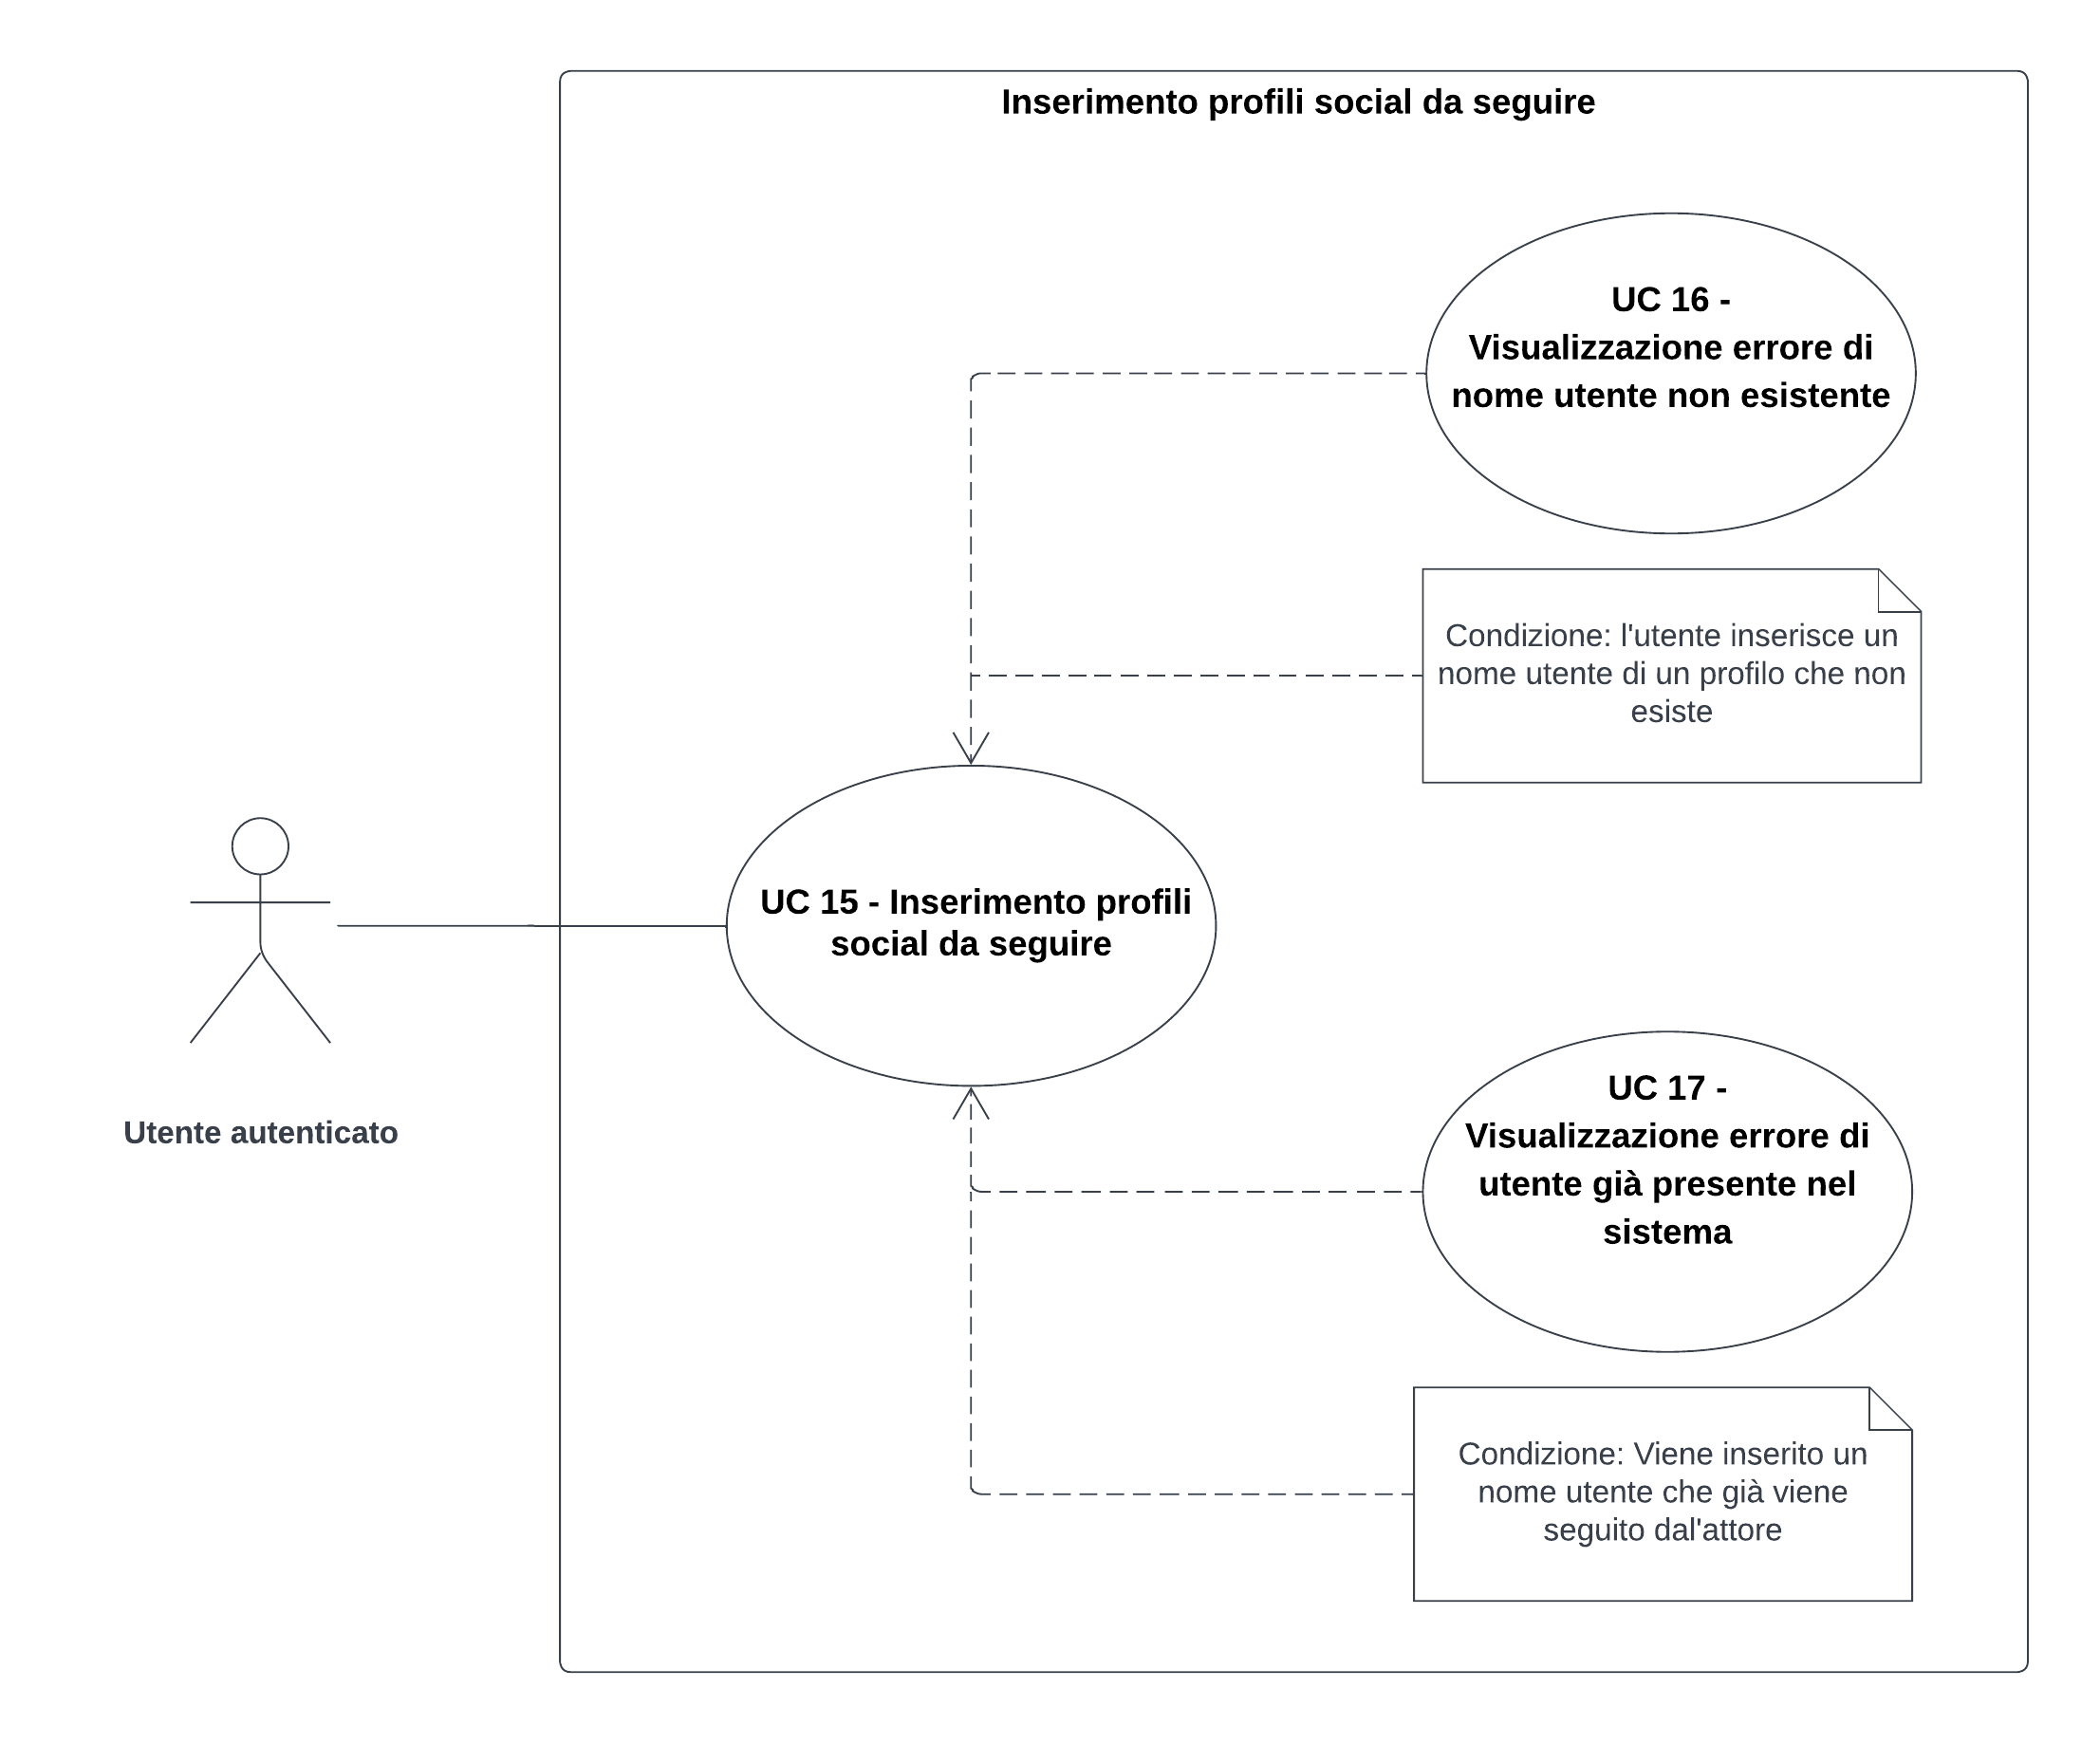
\includegraphics[width=15cm]{sezioni/Images/UC15.png}
    \centering
    \caption{Inserimento profili social da seguire}
\end{figure}

\begin{itemize}
    \item \textbf{Attore}: l'utente è autenticato.
    \item \textbf{Descrizione}: l'utente deve poter aggiungere dei profili social da seguire e da cui sarà generata la guida.
    \item \textbf{Scenario}:
    \begin{enumerate}
        \item l'utente naviga nella sezione dei profili seguiti;
        \item l'utente clicca il pulsante di aggiunta profilo;
        \item l'utente inserisce l'username da aggiungere;
        \item l'utente conferma e salva.
    \end{enumerate}
    \item \textbf{Estensioni}:
    \begin{itemize}
    	\item il profilo inserito non esiste \textbf{(UC17)};
    	\item il profilo inserito è già stato aggiunto \textbf{(UC18)}.
    \end{itemize} 
    \item \textbf{Precondizioni}: l'utente vuole seguire un nuovo utente.
    \item \textbf{Postcondizioni}: l'utente ha inserito un nuovo utente da seguire.
\end{itemize}

\subsection{UC17 - Visualizzazione errore di nome utente non esistente}
\begin{itemize}
    \item \textbf{Attore}: l'utente è autenticato.
    \item \textbf{Descrizione}: durante l'attività di aggiunta di un profilo l'utente deve ricevere un messaggio d'errore se il nome utente ricercato non è presente nel sistema.
    \item \textbf{Scenario}: l'utente legge un messaggio d'errore. 
    \item \textbf{Precondizioni}: l'utente inserisce un nome utente inesistente nella procedura di inserimento dei profili social da seguire.
    \item \textbf{Postcondizioni}: l'utente ha ricevuto un messaggio d'errore.
\end{itemize}

\subsection{UC18 - Visualizzazione errore di utente già presente nel sistema}
\begin{itemize}
    \item \textbf{Attore}: l'utente è autenticato.
    \item \textbf{Descrizione}: durante l'attività di aggiunta di un profilo l'utente deve ricevere un messaggio d'errore se il nome utente ricercato è già stato inserito nei profili seguiti dall'utente.
    \item \textbf{Scenario}: l'utente legge un messaggio d'errore. 
    \item \textbf{Precondizioni}: l'utente inserisce un nome utente nella procedura di inserimento dei profili social da seguire che è già presente tra quelli seguiti.
    \item \textbf{Postcondizioni}: l'utente ha ricevuto un messaggio d'errore.
\end{itemize}

\subsection{UC19 - Rimozione profili social seguito}

\begin{figure}[!h]
    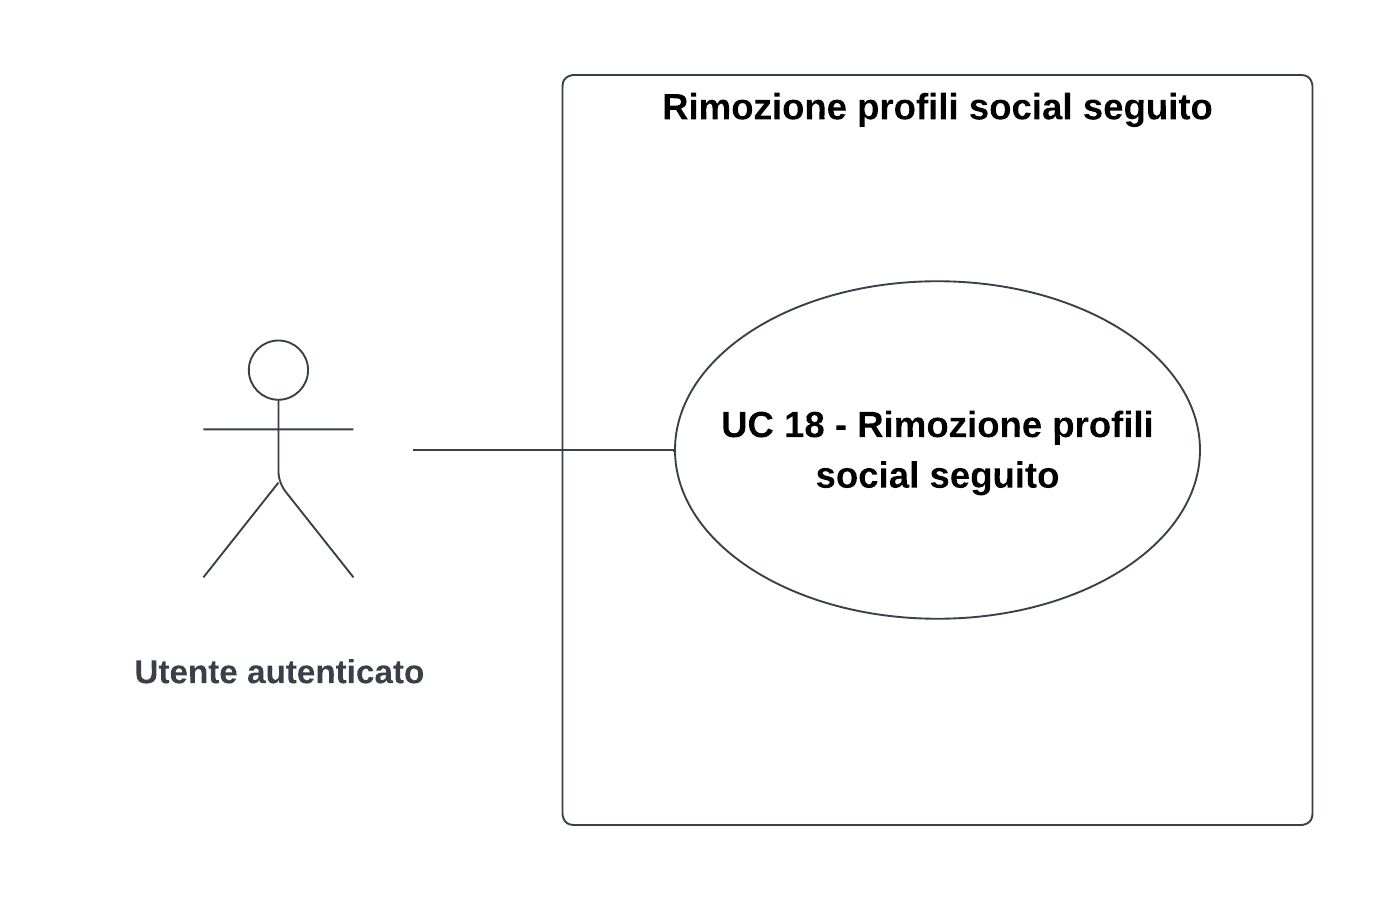
\includegraphics[width=10cm]{sezioni/Images/UC18.png}
    \centering
    \caption{Rimozione profili social seguito}
\end{figure}

\begin{itemize}
    \item \textbf{Attore}: l'utente è autenticato.
    \item \textbf{Descrizione}: l'utente deve poter rimuovere un profilo dalla lista di quelli seguiti.
    \item \textbf{Scenario}:
    \begin{enumerate}
        \item l'utente naviga nella sezione dei profili seguiti;
        \item l'utente seleziona il profilo che vuole rimuovere;
        \item l'utente clicca il pulsante di rimozione.
    \end{enumerate}

    \item \textbf{Precondizioni}: l'utente vuole rimuovere un profilo social dalla lista dei seguiti.
    \item \textbf{Postcondizioni}: l'utente ha rimosso il profilo social dalla lista dei seguiti.
\end{itemize}

\subsection{UC20 - Esplorazione profili social più seguiti}

\begin{figure}[!h]
    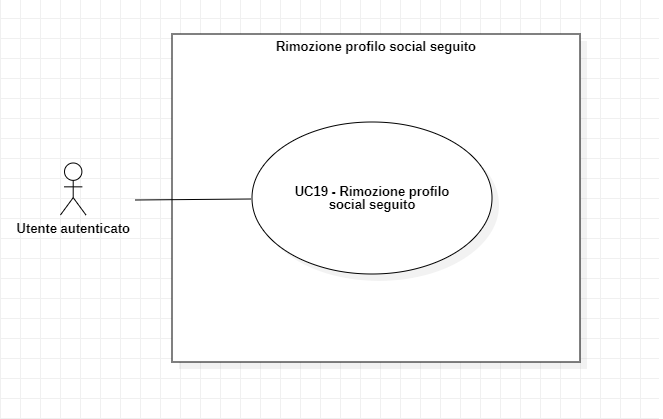
\includegraphics[width=10cm]{sezioni/Images/UC19.png}
    \centering
    \caption{Esplorazione profili social più seguiti}
\end{figure}

\begin{itemize}
    \item \textbf{Attore}: l'utente è autenticato.
    \item \textbf{Descrizione}: l'utente può esplorare i profili social più seguiti dagli altri utenti di questa piattaforma.
    \item \textbf{Scenario}:
    \begin{enumerate}
        \item l'utente si trova nella home;
        \item l'utente preme il pulsante per entrare nella pagina di esplorazione;
        \item l'utente vede la lista dei profili social più seguiti.
    \end{enumerate}
    \item \textbf{Precondizioni}: l'utente vuole visualizzare la lista dei profili social più seguiti.
    \item \textbf{Postcondizioni}: viene visualizzata all'utente la lista dei profili social più seguiti.
\end{itemize}

\subsection{UC21 - Impostazione vista predefinita guida}
\begin{figure}[!h]
    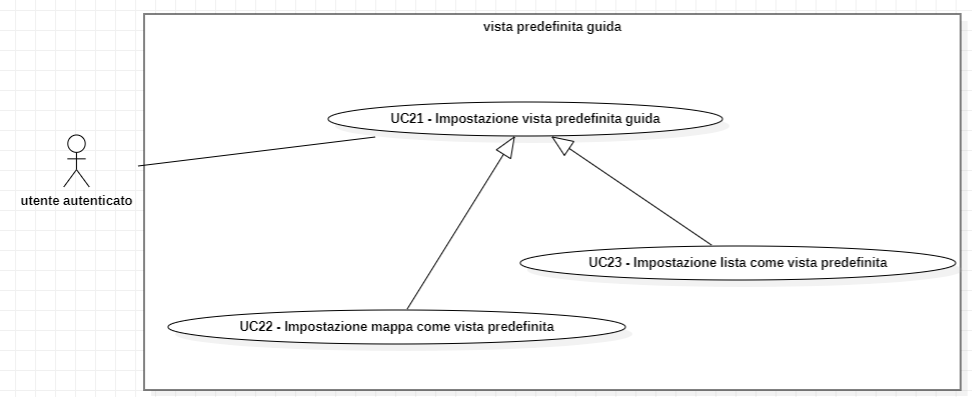
\includegraphics[width=15cm]{sezioni/Images/UC20_s.png}
    \centering
    \caption{Impostazione vista predefinita guida}
\end{figure}

\begin{itemize}
    \item \textbf{Attore}: l'utente è autenticato.
    \item \textbf{Descrizione}: l'utente deve poter scegliere la vista predefinita per visualizzare la guida.
    \item \textbf{Scenario}:
    \begin{enumerate}
        \item l'utente naviga nella sezione impostazioni;
        \item l'utente sceglie la voce “Vista predefinita”;
        \item l'utente sceglie tra la visulizzazione della mappa \textbf{(UC 22)} oppure della lista \textbf{(UC 23)}.
    \end{enumerate}

    \item \textbf{Precondizioni}: l'utente vuole poter sceglie la vista predefinita.
    \item \textbf{Postcondizioni}: la scelta della lista predefinita è stata salvata.
\end{itemize}

\subsection{UC22 - Impostazione mappa come vista predefinita}
\begin{itemize}
    \item \textbf{Attore}: l'utente è autenticato.
    \item \textbf{Descrizione}: l'utente sceglie la mappa come vista predefinita.
    \item \textbf{Scenario}: l'utente sceglie mappa come vista predefinita.
    \item \textbf{Precondizioni}: l'utente vuole scegliere mappa come vista predefinita.
    \item \textbf{Postcondizioni}: mappa viene impostata come vista predefinita.

\end{itemize}

\subsection{UC23 - Impostazione lista come vista predefinita}
\begin{itemize}
    \item \textbf{Attore}: l'utente è autenticato.
    \item \textbf{Descrizione}: l'utente sceglie la lista come vista predefinita.
    \item \textbf{Scenario}: l'utente sceglie lista come vista predefinita.
    \item \textbf{Precondizioni}: l'utente vuole scegliere lista come vista predefinita.
    \item \textbf{Postcondizioni}: lista viene impostata come vista predefinita.
\end{itemize}





